\documentclass[11pt,a4paper]{ivoa}
\input tthdefs

\newcommand{\xtype}[1]{\texttt{#1}}

\usepackage{listings}
\lstloadlanguages{XML,sh}
\lstset{flexiblecolumns=true,basicstyle=\small,tagstyle=\ttfamily}
\usepackage[utf8]{inputenc}
\usepackage{todonotes}
\usepackage{textcomp}
\usepackage{float}

\title{IVOA Dataset Access Protocol}

\ivoagroup{Data Access Layer Working Group}

\author{Patrick Dowler}
\author{Douglas Tody}
\author{Fran\c cois Bonnarel}
\author{Gregory Dubois-Felsnmann}

\editor{Patrick Dowler, Fran\c cois Bonnarel, Gregory Dubois-Felsmann}

\previousversion{}

\begin{document}
\begin{abstract}

The Dataset   Access protocol (DAP) provides capabilities for the discovery, description, access, and retrieval of dataproducts, including spectra, timeseries, visibility data,
2-D images as well as datacubes of three or more dimensions.  DAP data discovery is based on the ObsCore Data Model (ObsCoreDM, \cite{std:OBSCORE}), which primarily describes
data products by the physical axes (spatial, spectral, time, and polarization). Image datasets with dimension greater than 2 are often referred to as \textit{datacubes},
\textit{cube} or \textit{image cube} datasets and may be considered examples of \textit{hypercube} or \textit{n-cube} data.  In this document the term “image” refers to general
multi-dimensional datasets and is synonymous with these other terms unless the image dimensionality is otherwise specified. \\
DAP provides capabilities for dataset discovery and access. Data discovery and  metadata access (using ObsCoreDM) are defined here. The capabilities for drilling down 
to data files (and related resources) and services for remote access are defined elsewhere, but DAP also allows for direct access to retrieval. 

\end{abstract}
\section*{Acknowledgments}
The authors would like to thank all the participants in DAL-WG discussions  for their ideas, critical reviews, and contributions to this document.

\section{Introduction}

The Dataset Access (DAP) protocol defines several capabilities to support discovery and access to astronomical datasets of any type and dimension.  Typical datasets include 
spectra, timeseries, 2-D spatial images, spectral data cubes, and cube and hypercube data of higher dimensions as well as derived image data products an event list or
visibility data.  The underlying ObsCore data model is a simplified view on the typical image datasets derived from observational data, which have some combination of
spatial, spectral (including velocity and redshift), time, and polarization axes.  
For complete access to datacubes, the SIA-2.0 specification  makes use of features defined in DataLink \citep{std:DataLink}. It also makes use of AccessData services such
as SODA \citep{2017ivoa.spec.0517B}, as well as custom data services.




\begin{figure}[H]
\centering

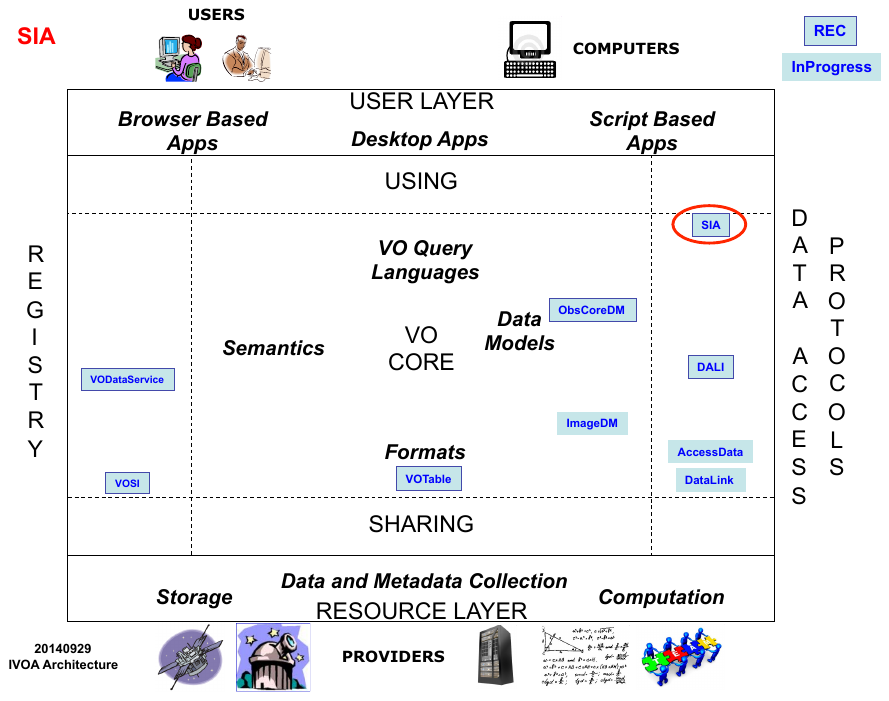
\includegraphics[width=0.9\textwidth]{archdiag.png}
\label{fig:architecture}
\end{figure}


DAP defines data discovery and metadata capabilities that work with other DAL services to enable image, data cube and other types of dataset access. 
The basic interface for the capabilities defined in this specification are described in DALI \citep{std:DALI}. DataLink can be used with DAP for finding access URL(s) for files,
related resources, and data services such as SODA. DAP services also support VOSI-availability and VOSI-capabilities \citep{std:VOSI}  resources.




The ObsCore data model has been defined in \cite{std:OBSCORE}, it contains and organizes the minimal set of metadata necessary to discover datasets of interest for
a specific purpose. The metadata returned from the DAP data discovery request is defined by the ObsCore data model and serialized according to the ObsTAP specification
\citep{std:OBSCORE}; this may be extended with additional metadata (columns)  in the future. Data discovery responses are returned in VOTable \citep{std:VOTABLE} format 
unless an alternate format is requested.


\subsection{The Role in the IVOA Architecture}


DAP specifies standardID values for each capability, as defined by VODataService \citep{std:VODS11}. DAP services may be registered in an IVOA Registry using the SimpleDALRegExt \citep{std:DALREGEXT} extension schema.
\subsection{Changes from SIA-2.0 to DAP}



Virtual Observatory access to astronomical images has been available via the SIA-1.0 protocol for over a decade.  
Many such services have been implemented since 2002, and SIA-1.0 \citep{std:SIAP} was formally standardized as an IVOA Recommendation in 2009. 
SSA \citep{std:SSAP} played a similar role for spectra and also used specific metadata in the query response. 
SIA-2.0 \citep{std:SIAv2} was multi-dimensional and fully integrated with the modern VO architecture and related 
standards, but restricted to images and data cubes.
DAP is an extension of SIA2 to other dataproduct types. It can be seen as a server side  parameter based proxy to an ObsTAP service.

\subsection{Motivating Use Cases}

Below are some of the more common use cases that have motivated the development of the DAP specification. 
While this is not complete, it helps to understand the problem area covered by this specification.

\subsubsection{Simple Data Discovery}

Simple data discovery entails finding services that provide parameter based discovery of images and datacubes, querying the service(s) with a few well known kinds of queries 
that cover greater than 95\% of use, and getting back easily parsed summary metadata about each available data product. The service discovery would be performed with an
IVOA Registry search using a new service type defined for DAP. 


The query for data would need to allow for querying in position, energy, time, and polarization:
\begin{itemize}
    \item find data that includes specified coordinates (e.g. for some object)
    \item find data in the circle with coordinate centre and radius
    \item find data in a range of longitude and latitude
    \item find data within a specified simple  polygon (one region, no holes, less than half the sphere)
    \item find data containing a specified energy (e.g. wavelength) or in a specified range of energy values
    \item find data obtained at a specified time (e.g. including a time instant) or during a specified range of times
    \item find data obtained with specified polarization (Stokes) states
    \item find data within a specified range of spatial resolution
    \item find data within a specified range of field-of-view
    \item find data within a range of exposure (integration) time
    \item find data of a specific dataproduct\_type	    

\end{itemize}
Queries can also combine any of these kinds of constraints (e.g. query using
position and energy, position and time, etc.). Queries should be easily formulated with parameter-value pairs.

\subsubsection{Get Detailed Metadata}

The data discovery phase returns a subset of the available metadata.  Clients may need additional detailed metadata (as defined by any IVOA Data model specification) in order
to make decisions or perform computations required to access the data (e.g. using a separate low-level data access service as described in the SODA specification). The client
must be able to easily figure out if detailed metadata is available and, using an identifier from the discovery response, make a call to a web service to retrieve the detailed metadata.

\subsubsection{Download Complete Datasets}
\label{sec:sync}

The client should be able to download complete datasets with information available in the discovery response. If the dataset is a single file, the service should provide an
access URL to the file; if it is multiple files, then an access URL to a DataLink service [9] can be provided, but the client must be able to easily distinguish these two scenarios.


\subsubsection{Access a Dataset with Operations: Too Big to Download}

\label{sec:async}

In many cases, datasets are too large to download and process locally, so the client must be able to perform remote operations.
Data discovery could be performed using any discovery protocol (DAP, SIA, TAP with ObsCore, etc.).
The client must be able to easily figure out if a low level access service is available for a discovered dataset. 
This could be using a URL provided in the response or by calling an associated DataLink service.
Access operations include basic filtering (cut out a subsection of the data), transformations, 
or other pixel-level operations or even analysis. With version 1.0 of the SODA  specification, we only cover
extracting a simple subset of an image or datacube. 


\subsection{Scope and Related Documents}
\label{sec:examples}


Some of the support for these use cases is provided by the separate capabilities defined in the DataLink and SODA specifications. Together, these three specifications,
plus TAP \citep{std:TAP}, and  within the framework provided by ObsCore, and the future cube data model provide a set of capabilities required to support a broad range of use cases.



\begin{figure}[H]
\centering

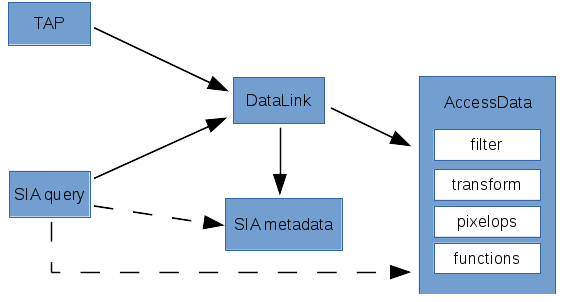
\includegraphics[width=0.9\textwidth]{schema.png}
\label{fig:architecture}
\end{figure}



Each box in the above diagram shows a single capability. The DAP query capability is defined in this specification; the SIA metadata capability is defined in a later version
of the SODA specification, supported by the Cube DM specification. DataLink  and SODA are separate specifications. The dashed lines represent optimisations that are mentioned
in use cases above, where subsequent service usage should be easy to discover and invoke.





\section{Resources}
\label{sec:parameters}

The DAP data discovery capability is implemented as a synchronous resource conforming to the DALI-sync  specification.


\begin{table}[H]
\begin{tabular}{lll}
\sptablerule
\textbf{resource type}&\textbf{resource name}&\textbf{required}\cr
\sptablerule

\texttt{\{query\}}&\texttt{service specific}&{yes}\cr
\texttt{DALI-examples}&\texttt{/examples}&\texttt{no}\cr
\texttt{VOSI-availability}&\texttt{/availability}&\texttt{yes}\cr
\texttt{VOSI-capabilities}&\texttt{/capability}&\texttt{yes}\cr
\sptablerule
\end{tabular}
\caption{DALI specification of SIA resources}
\label{tab:DALIspec}
\end{table}

A DAP service must have at least one \{query\} resource; it could have multiple \{query\} resources (e.g. to support alternate authentication schemes where the path is different).
All \{query\} resources must be siblings of the VOSI-capabilities resource; this limitation enables a client with just the URL for a DAP {query} resource (e.g. from a Datalink 
service descriptor) to find the VOSI-capabilities resource and discover all the capabilities provided.

\subsection{\{query\} resource}
\label{sec:query}
The \{query\} resource is a synchronous web service resource that conforms to the DALI-sync description. The implementer is free to name (set the path of) this resource however
they like; the client will find the resource path using the VOSI-capabilities resource. 

As a DALI-sync resource, the parameters for a request may be submitted using an HTTP GET (query string) or POST action.

All parameters for the \{query\} resource defined below must be supported by the service. Services must accept parameters and apply the constraints such that if a (ObsCore) record
does not satisfy the constraints it is not included in the response. If the metadata for a field is not known (null), the constraint cannot be satisfied. The ObsCore data model
defines which fields may be null and which must have a value. For example, if dataset(s) have unknown time coverage (t\_min and t\_max in ObsCore), a query with the TIME 
parameter must not return the record(s); queries without the TIME constraint could still return such records, so the caller can discover such dataset(s).

Client requests may include zero or more of the query parameters.

All query parameters are multi-valued which means multiple occurrences of the parameter=value pairs as specified in the DALI recommendation are permitted. The constraints from
multiple occurrences of a parameter are combined with a logical OR operator. The constraints from different parameters are combined with a logical AND operator.

Query parameters for numeric fields accept a single floating point value or a range of values with optional lower and upper bounds. Such range values are encoded using the VOTable
array serialisation (space separated). If  the lower or upper bound is not specified, the range is open-ended. In VOTable arrays this uses the special values -Inf or +Inf. 
For example, the interval [300,600] is:

\begin{lstlisting}
300 600 
\end{lstlisting}
The open-ended interval [300,infinity) (all values greater than or equal to 300) is:

\begin{lstlisting}
 300 +Inf 
\end{lstlisting}
The open-ended interval (-infinity,600] (all values less than or equal to 600) is:

\begin{lstlisting}
 -Inf 600 
\end{lstlisting}
 The open-ended interval (-infinity,infinity) (all values) is: 

\begin{lstlisting}
 -Inf +Inf 
\end{lstlisting}
If specified, the boundary value is always included in the interval.
The units for numeric values are specified for each parameter and never included in the value.
 
Except where explicitly noted (see for example~\ref{sec:ID}), query parameters for text or string fields are always case-sensitive and indicate an exact match. Wild carding is not allowed
except where explicitly noted (see again ~\ref{sec:ID}). In other string-valued parameters multiple occurence of the same parameter should be used instead.
The sections describing query parameters make use of fixed reference systems and units to simplify client and service implementation. These choices are not suitable for all domains;
the values are chosen to enable the {query} resource to be used to search for most standard observational astronomy data. If they are not suitable for a specific domain of interest
(e.g. planetary science) then it is feasible to write a very short standard that re-uses the DAP {query} capability but redefines the hard-coded systems and units. This new standard
would have a new standardID to distinguish services that implement it from those that implement the capability defined here.



\subsubsection{MOC}
The MOC parameter defines a spatial, temporal or combination of both subset of space-time to be searched using the \xtype{moc} defined in DALI. The parameter syntax is defined as in
the MOC specification \citep{MOC2}


Examples :
\begin{itemize}

\item Searching in cells 1 and 2 at order 1 will read this way MOC = 1/1 2
\item Searching in cells 1 at order 1 and cells 1 to 6 at order 2 will read MOC = 1/1 2/1-6
\item Searching in time cell 1 at order 61 in in combination with spatial cells 0 to 2 at order 29 will read this way MOC = t61/1 s29/0-2 	

\end{itemize}


\subsubsection{POS}
\label{sec:POS}

The POS parameter defines the positional region(s) to be searched for data. The value is made up of a shape keyword followed by coordinate values. A POS constraint is satisfied if 
the specified shape intersects the bounds (s\_region in the ObsCore data model) of the observation. 
 The allowed shapes are:
\begin{table}[H]
\begin{tabular}{ll}
\sptablerule
\textbf{Shape}&\textbf{Coordinate values}\cr
\sptablerule
\texttt{CIRCLE}&\texttt{<longitude> <latitude> <radius>}\cr
\texttt{RANGE}&\texttt{<longitude1> <longitude2> <latitude1> <latitude2>}\cr
\texttt{POLYGON}&\texttt{<longitude1> <latitude1> ... (at least 3 pairs)}\cr
\sptablerule
\end{tabular}
\caption{POS Values in Spherical Coordinates}
\label{tab:shapetypes}
\end{table}
A circle at (12,34) with radius 0.5:

\begin{lstlisting}
POS=CIRCLE 12.0 34.0 0.5
\end{lstlisting}
A range of [12,14] in longitude and [34,36] in latitude: 

\begin{lstlisting}
POS=RANGE 12.0 12.5 34.0 36.0 
\end{lstlisting}
A polygon from (12,34) to (14,35) to (14,36) to (12,35) and (implicitly) back to (12,34): 

\begin{lstlisting}
POS=POLYGON 12.0 34.0 14.0 35.0 14. 36.0 12.0 35.0
\end{lstlisting}

The inside is always assumed to be the smaller of the region to the left and the region to the right so only polygons smaller than half the sphere can be specified. \\ \\
A band around the equator: 

\begin{lstlisting}
POS=RANGE 0 360.0 -2.0 2.0 
\end{lstlisting}
The north pole: 

\begin{lstlisting}

POS=RANGE 0.0 360.0 89.0 90.0 

\end{lstlisting}
Although it is not really useful, the whole sky can be expressed:



\begin{lstlisting}

POS=RANGE 0.0 360.0 -90.0 90.0

\end{lstlisting}


This syntax for circles and polygons is in the same style as STC-S, but with no reference positions, coordinate systems, units, or geometric operators (union, intersection, not).
Coordinate values are floating point right ascension (RA) and declination (DEC) in ICRS and the units are always degrees. Valid coordinate values are in [0,360] for longitude 
and [-90,90] for latitude (or NaN).

\subsubsection{BAND}
\label{sec:BAND}

The BAND parameter defines the energy interval(s) to be searched for data. The value is an open or closed energy interval. The interval always includes the bounding values. 
A BAND constraint is satisfied if the interval intersects the energy coverage of the observation ([em\_min,em\_max] in the ObsCore data model). \\ \\
Find data with spectral coverage that overlaps 500 to 550nm:

\begin{lstlisting}
BAND=500e-9 550e-9
\end{lstlisting}
Find data with wavelength longer than 300m:
\begin{lstlisting}
BAND=300 +Inf
\end{lstlisting}
Find data with wavelength shorter than 21cm:
\begin{lstlisting}
BAND=-Inf 0.21
\end{lstlisting}
Find data that includes 21cm:
\begin{lstlisting}
BAND=0.21
\end{lstlisting}
The scalar value 550, equivalent to [550,550]:
\begin{lstlisting}
BAND=550
\end{lstlisting}


Searching using a scalar value should match any data that includes the specified value; searching using an interval will find any data with energy coverage that intersects 
the specified interval.

Energy values used in the BAND parameter are always assumed to be  observed wavelength in meters. The ObsCore data model does not define a specific reference frame for values of 
em\_min and em\_max; values in the BAND parameter are assumed to be in the same (unspecified) frame as the content (e.g. no specific frame or transformation should be assumed). 

\subsubsection{TIME}
\label{sec:TIME}

The TIME parameter defines the time interval(s) to be searched for data. The value is an open or closed interval with numeric values (interpreted as Modified Julian Dates). 
A TIME constraint is satisfied if the interval intersects the time coverage of the observation ([t\_min,t\_max] in the ObsCore data model).

A range of MJD values:

\begin{lstlisting}
TIME=55123.456 55123.466
\end{lstlisting}

An instant in time:

\begin{lstlisting}
TIME=55678.123456
\end{lstlisting}

Values used in the TIME parameter are always interpreted as specified in DALI in the section on literal values: UTC time scale and UNKNOWN reference position \citep{std:STC}. 
Modified Julian Date values are always in days.

\subsubsection{POL}
\label{sec:POL}

The POL parameter defines the polarization state(s) to be searched  for matching data.  \\ \\
Find data with unpolarized intensity:

\begin{lstlisting}
POL=I
\end{lstlisting}
Find data with standard circular polarization:

\begin{lstlisting}
POL=V
\end{lstlisting}
Find  right or left circular polarized data:

\begin{lstlisting}
POL=RR
POL=LL
\end{lstlisting}
Find data with any of IQU components:

\begin{lstlisting}
POL=I
POL=Q
POL=U
\end{lstlisting}

The POL parameter constrains values of the pol\_states column of the ObsCore data model; possible values for the POL parameter are also defined by ObsCore.

This parameter is case insensitive.



\subsubsection{FOV}

The FOV parameter defines the range(s) of field of view (size) to be searched for data. This constraint is satisfied if the specified range includes the size of the field of
view (s\_fov column of the ObsCore data model). \\ \\
Find data with field of view between 1 and 2 degrees:

\begin{lstlisting}
FOV=1.0 2.0
\end{lstlisting}
Find data with field of view larger than 1.0 degrees:

\begin{lstlisting}
FOV=1.0 +Inf
\end{lstlisting}
Find data with field of view smaller than ~1 arcmin:

\begin{lstlisting}
FOV=-Inf 0.017
\end{lstlisting}
Find data with very small (< 0.01 deg) or very large (> 2 deg) field of view:

\begin{lstlisting}
FOV=-Inf 0.01
FOV=2.0 +Inf
\end{lstlisting}

Values used in the FOV parameter are always interpreted as angles expressed in degrees (same units as the s\_fov column in the ObsCore data model).

\subsubsection{SPATRES}

The SPATRES parameter define the range(s) of spatial resolution to be searched for data. This constraint is satisfied if the specified range includes the spatial resolution 
of the data (s\_resolution column of the ObsCore data model). \\ \\
Find data with resolution better than 0.2 arcsec:

\begin{lstlisting}
SPATRES=-Inf 0.2
\end{lstlisting}
Find data with resolution larger than 1.0 arcsec:

\begin{lstlisting}
SPATRES=1.0 +Inf 
\end{lstlisting}
Find data with resolution between 0.1 and 0.2 arcsec:

\begin{lstlisting}
SPATRES=0.1 0.2
\end{lstlisting}

Values used in the SPATRES parameter are always interpreted as angles expressed in arcsec (same units as the s\_resolution column in the ObsCore data model).

\subsubsection{SPECRP}

The SPECRP parameter define the range(s) of spectral resolving power to be searched for data. This constraint is satisfied if the specified range includes the resolving power
of the data (em\_res\_power column of the ObsCore data model). \\ \\
Find data with resolution better than 1000:

\begin{lstlisting}
SPECRP=1000 +Inf
\end{lstlisting}
Find data with resolution less than 500:

\begin{lstlisting}
SPECRP=-Inf 500
\end{lstlisting}
Find data with resolution between 10000 and 20000:

\begin{lstlisting}
SPECRP=10000 20000
\end{lstlisting}


Values used in the SPECRP parameter are dimensionless ($\lambda$/$\Delta$$\lambda$, as for the em\_res\_power column in the ObsCore data model).

\subsubsection{EXPTIME}

The EXPTIME parameter defines the range(s) of exposure times to be searched for data. This constraint is satisfied if the specified range includes the exposure time of 
the data (t\_exptime column of the ObsCore  data model). \\ \\
Find data with exposure time less than  60 seconds:

\begin{lstlisting}
EXPTIME=-Inf 60
\end{lstlisting}
Find data with exposure time longer than 10 minutes:

\begin{lstlisting}
EXPTIME=600 +Inf
\end{lstlisting}
Find data with exposure time between 10 and 30 minutes:

\begin{lstlisting}
EXPTIME=600 1800
\end{lstlisting}
Find data with very short (< 2 sec) or very long (> 20 min) exposure time:

\begin{lstlisting}
EXPTIME=-Inf 2
EXPTIME=1200 +Inf
\end{lstlisting}


Values used in the EXPTIME parameter are always expressed in seconds (same units as the t\_exptime column in ObsCore).

\subsubsection{TIMERES}
The TIMERES parameter define the range(s) of temporal resolution to be searched for data. This constraint is satisfied if the specified range includes the temporal resolution of 
the data (t\_resolution column of the ObsCore data model). \\ \\
Find data with resolution better than 1.0 sec:

\begin{lstlisting}
TIMERES=-Inf 1.0
\end{lstlisting}
Find data with resolution larger than 1.0 sec:

\begin{lstlisting}
TIMERES=1.0 +Inf
\end{lstlisting}
Find data with resolution between 1.0 and 2.0 sec:

\begin{lstlisting}
TIMERES=1.0 2.0
\end{lstlisting}

Values used in the TIMERES parameter are always expressed in seconds (same units as the t\_resolution column in the ObsCore  data model).

\subsubsection{ID}
\label{sec:ID}

The ID parameter is a string-valued parameter that specifies the identifier of dataset(s). Values of the ID parameter are compared to the obs\_publisher\_did column of the ObsCore data model. 
Note that IVOIDs MUST be compared case-insensitively. As publisher dataset identifiers in the VO generally are IVOIDs, implementations will usually have to use case-insensitive comparisons here.
When wildcarding of the end of the  ID is needed the expression "extensionof ivo://bla" SHOULD be used.


\subsubsection{COLLECTION}

The COLLECTION parameter is a string-valued parameter that specifies the name of the data collection. The value is compared with the obs\_collection from the ObsCore  data model.


\subsubsection{FACILITY}

The FACILITY parameter is a string-valued parameter that specifies the name of the facility (usually telescope) where the data was acquired. The value is compared with the facility\_name 
from the ObsCore data model.


\subsubsection{INSTRUMENT}
The INSTRUMENT parameter is a string-valued parameter that specifies the name of the instrument with which the data was acquired. The value is compared with the instrument\_name from the
ObsCore data model.

\subsubsection{DPTYPE}


The DPTYPE parameter is a string-valued parameter that specifies the type of data. This parameter is case-insensitive. The value is compared with the dataproduct\_type from the ObsCore data
model.  In contrast to SIA2.0 which allows only dataproduct\_types  \textit{image} and \textit{cube}, all the other dataproduct\_types are allowed, in such a way that we can constrain the
service to retrieve visibility data, timeseries and event lists. Using DPTYPE with the "spectrum" value can be considered as an upgrade of the SSA protocol.

ObsCore extension have been defined for visibility data and TimeSeries. It is possible to query services using these extensions by optional query parameters defined in Appendix B.


\subsubsection{CALIB}
The CALIB parameter is a integer-valued parameter that specifies the calibration level of the data. The value is compared with the calib\_level from the ObsCore data model. To find raw data:

\begin{lstlisting}
CALIB=0
CALIB=1
\end{lstlisting}
To find calibrated data:

\begin{lstlisting}
CALIB=2
\end{lstlisting}
To find calibrated data and more highly processed data products:

\begin{lstlisting}
CALIB=2
CALIB=3
\end{lstlisting}

\subsubsection{TARGET}

The TARGET parameter is a string-valued parameter that specifies the name of the target (e.g. the intention of the original science program or observation). The value is compared with the
target\_name from the ObsCore data model. This parameter is case sensitive.


\subsubsection{FORMAT}

The FORMAT parameter specifies the  format returned by  the access  link.  The value is compared with the access\_format column from the ObsCore data model when this one contains a dataset MIME type. 
In that case this column describes the format of the response from the access\_url (see 3.1.3) so the values could be data file types (e.g. application/fits).  In case access\_format contains  the DataLink  MIME type (\cite{std:DataLink}, \cite{std:TSV}) the FORMAT parameter value constrains the content_type value for the #this items in the DataLink response.
This parameter is case insensitive.

\subsubsection{RELEASEDATE}
The RELEASEDATE parameter specifies the range of release dates to be searched for data. 
The limits are compared to the obs\_release\_date optional attribute of the ObsCore data model. 
They are expressed as 2 ISO 8601 dates in the general case. A single value is searched for an exact match.
As the obs\_release\_date attribute is optional, the service self description (\ref{sec:selfdesc})  informs the user of the availability of this parameter.
RELEASEDATE queries for services not providing the release\_date attribute SHOULD provide an empty response.



%\subsubsection{RETRIEVEMODE (2 solutions)}
%This parameter is case-insensitive.
%\begin{itemize}


%\item solution 1 : The RETRIEVEMODE parameter allows to select between the full retrieval of the discovered dataset (RETRIEVEMODE = FULL) and a cutout operated by SODA (RETRIEVEMODE = CUTOUT). 
%The default value is "FULL". This parameter allows to find back the distinction operated by SIA1.0 between the archive and cutout modes. 
%SIA2.0 missed this parameter. The SIA2.0 service behavior was supposed to allow only direct full retrieval of datasets or to retrieve DataLink responses.
%In the "CUTOUT" case the access\_url is a SODA query using the same input parameters than the SIA query. In these conditions coverage parameters POS, CIRCLE, POLYGON, BAND, TIME, POL,
%specify both the search area and the subset of data to be extracted.  


%\item solution 2 : The RETRIEVEMODE parameter allows to select between the full retrieval of the discovered dataset (RETRIEVEMODE = FULL) and a cutout operated by SODA (RETRIEVEMODE = CUTOUT). 
%SODA Service descriptors may be added to the SIA query response. In the "RETRIEVEMODE = CUTOUT" case the SODA service descriptor input parameters are predefined by the SIA input parameters.
%To get the discovered cutout the user simply has to validate the SODA activate button in her favorite VO client. In the default   (RETRIEVEMODE = FULL) case the SODA interface will prompt 
%the user for interactively defined values.
%\end{itemize}
\subsubsection{MAXREC}
The MAXREC parameter is defined in DALI and allows the client to limit the number or records in the response. A service implementation may also impose default and maximum values for this limit.
However the limit is determined, if the output is truncated due to the limit the server must indicate this using an overflow  (section~\ref{sec:succesful}) indicator except in the the special 
case of MAXREC=0, where the  service respond with metadata-only (normal output document with no records).


\subsubsection{UPLOAD}

 
 The DALI UPLOAD parameter is not used by this version of DAP. The use case of uploading lists of coordinates is covered by the multiple-valued parameters values.


\subsubsection{Service PARAMETER self description}

\label{sec:selfdesc}
Any service SHOULD  include a DataLink service descriptor in the VOTable output to describe itself. 
This descriptor would describe the supported query parameters (standard and custom), including list 
of values for those with a fixed list (COLLECTION, INSTRUMENT, FACILITY, DPTYPE, CALIB, and FORMAT).
This is particularly important for those parameters where the fixed list is not standardized by any
specification such as COLLECTION, INSTRUMENT and FACILITY.


\subsection{Availability: VOSI-availability}

A web service with DAP capabilities must have a VOSI-availability resource \citep{std:VOSI}  as described in DALI .

\subsection{Capabilities: VOSI-capabilities}

A web service with DAP capabilities must have a VOSI-capabilities resource \citep{std:VOSI} as described in DALI . The standardID for the \{query\} capability is 

\begin{lstlisting}

ivo://ivoa.net/std/DAP#query-1.0

\end{lstlisting}

All DAL services must implement the /capabilities resource. The following capabilities document shows the minimal metadata and does not require a registry extension schema:

\begin{lstlisting}[language=XML]


<?xml version="1.0" encoding="UTF-8"?>
<vosi:capabilities 
   xmlns:vosi="http://www.ivoa.net/xml/VOSICapabilities/v1.0" 
   xmlns:xsi="http://www.w3.org/2001/XMLSchema-instance" 
   xmlns:vs="http://www.ivoa.net/xml/VODataService/v1.1">
  <capability standardID="ivo://ivoa.net/std/VOSI#capabilities">
    <interface xsi:type="vs:ParamHTTP" version="1.0">
      <accessURL use="base">
         http://example.com/dap/capabilities
      </accessURL>
    </interface>
  </capability>
  <capability standardID="ivo://ivoa.net/std/VOSI#availability">
    <interface xsi:type="vs:ParamHTTP" version="1.0">
      <accessURL use="full">
         http://example.com/dap/availability
      </accessURL>
    </interface>
  </capability>
  <capability standardID="ivo://ivoa.net/std/SIA#query-2.0">
    <interface xsi:type="vs:ParamHTTP" role="std" version="2.0">
      <accessURL>
           http://example.com/dap/query
      </accessURL>
    </interface>
    <!-- service details from extension schema could go here -->
  </capability>
</vosi:capabilities>
\end{lstlisting}

Note that the {query} resource does not have to be named as shown in the accessURL(s) above. Multiple capability elements for the {query} and the {metadata} resources may be included; 
this is typically used if they differ in protocol (http vs. https) and/or authentication requirements.

\section{\{query\} response}
\label{sec:queryresponse}

\subsection{Successful Query}
\label{sec:succesful}

The response from a successful call to the \{query\} resource is a table consistent with  ObsTAP responses as described in \cite{std:OBSCORE}. The ObsCore data model specifies all the (VOTable)
field names, utypes, UCDs, and units to use in the response, as well as which fields must have values and which are allowed to be empty (null). The \{query\} response must contain the required 
ObsCore fields and may contain additional fields (from ObsCore or custom fields from the service provider). Examples are provided below (section~\ref{sec:Examples}).

Successfully executed requests should result in a response with HTTP status code 200 (OK) and a response in the format requested by the client or in the default format for the service. 
The default output format is VOTable. Other output formats can be specified by the RESPONSEFORMAT parameter (see \cite{std:DALI}).

The service should set the following HTTP headers to the correct values where possible.
\begin{table}[H]
\begin{tabular}{ll}
\sptablerule
\textbf{Content-Type}&\textbf{mime-type of the response}\cr
\sptablerule
\texttt{Content-Encoding}&\texttt{encoding/compression of the response (if applicable)}\cr
\sptablerule
\end{tabular}
\caption{Recommended HTTP Response Headers}
\label{tab:RespHead}
\end{table}





Since the \{query\} response is usually dynamically generated, the Content-Length and Last-Modified headers cannot usually be set.

\subsubsection{Related Service Metadata}
The DataLink specification  gives a recipe for including additional resources in VOTable that enable the client to invoke services using values from the table as parameter values. 

If the provider implements a DataLink service for the data being found via DAP, the \{query\} response should include a description for invoking the DataLink service, usually using
values from the obs\_publisher\_did column.

 

If the provider implements a SODA capability for the data being found via DAP and this capability can be invoked directly using an identifier in the \{query\} response,
the \{query\} response should include a description for invoking this capability, usually using values from the obs\_publisher\_did column.





\subsubsection{DAP {query} Service Descriptor}



The DataLink specification describes a mechanism for describing a service within a VOTable resource and recommends that services can describe themselves with a special resource with name="this".
DAP \{query\} responses should include a descriptor describing both standard and custom query parameters (if applicable). The descriptor for a service with standard parameters 
(see~\ref{sec:query}) would be:

\begin{lstlisting}[language=XML]
<RESOURCE type="meta" utype="adhoc:service" name="this">
 <PARAM name="standardID" datatype="char" arraysize="*"
        value="ivo://ivoa.net/std/DAP#query-2.0" />
 <PARAM name="accessURL" datatype="char" arraysize="*"
        value="http://example.com/dap/query" />
 <GROUP name="inputParams">
  <PARAM name="POS" datatype="char" arraysize="*" xtype="circle" />
  <PARAM name="POS" datatype="char" arraysize="*" xtype="range" />
  <PARAM name="POS" datatype="char" arraysize="*" xtype="polygon" />
  <PARAM name="BAND" datatype="double" arraysize="*" 
         xtype="interval" unit="m" />
  <PARAM name="TIME" datatype="double" arraysize="*" 
         xtype="interval" unit="d" />
  <PARAM name="POL" datatype="char" arraysize="*" />
  <PARAM name="FOV" datatype="double" arraysize="*" 
         xtype="interval" unit="deg" />
  <PARAM name="SPATRES" datatype="double" arraysize="*" 
         xtype="interval" unit="arcsec" />
  <PARAM name="EXPTIME" datatype="double" arraysize="*" 
         xtype="interval" unit="sec" />
  <PARAM name="ID" datatype="char" arraysize="*" />
  <PARAM name="COLLECTION" datatype="char" arraysize="*" />
  <PARAM name="FACILITY" datatype="char" arraysize="*" />
  <PARAM name="INSTRUMENT" datatype="char" arraysize="*" />
  <PARAM name="DPTYPE" datatype="char" arraysize="*" />
  <PARAM name="CALIB" datatype="int" />
  <PARAM name="TARGET" datatype="char" arraysize="*" />
  <PARAM name="TIMERES" datatype="double" arraysize="*" 
         xtype="interval" unit="sec" />
  <PARAM name="SPECRP" datatype="double" arraysize="*" 
         xtype="interval" />
  <PARAM name="FORMAT" datatype="char" arraysize="*" />

 </GROUP>
</RESOURCE>

\end{lstlisting}
This VOTable resource should be included in the output from all queries; it is especially useful for MAXREC=0 queries since inclusion of the self descriptor would mean that all inputs and 
outputs would be fully described.




\subsubsection{Use of access\_url and access\_format}

If the DAP service is only dealing with simple data (one file per result), the access\_url column may be a link directly to that file, in which case the access\_format column should specify
the file format (e.g. application/fits). 


If the data provider implements a DataLink service for the data being found via the SIA {query} capability, they may put a URL to invoke the DataLink {links} capability (with ID parameter and 
value) in the access\_url column; if they do this, they must also put the standard DataLink MIME type in the access\_format column.





\subsection{Errors}
\label{sec:error-codes}
The error handling specified for DALI-sync resources applies to service failure. If the requested format is VOTable, the error document must be VOTable as described by DALI, except when 
the service is broken.  If the requested format is one of the plain text (csv or tsv) formats, the error document should also be plain text using the text/plain content-type.
The error message must start with one of the strings in the following table, in order of specificity:

\begin{table}[H]
\begin{tabular}{ll}
\sptablerule
\textbf{Error}&\textbf{Meaning}\cr
\sptablerule
UsageFault&Invalid input (e.g. invalid input parameter value\cr
\sptablerule
TransientFault&Service is not currently able to function\cr
\sptablerule
FatalFault&Service cannot perform requested action\cr
\sptablerule
DefaultFault&General error (not covered above)\cr
\end{tabular}
\caption{Error Messages}
\label{tab:ErrMess}
\end{table}

In all cases, the service may append additional useful information to the error strings above. If there is additional text, it must be separated from the error string with a colon (:) character,
for example:
\begin{lstlisting}
UsageFault: invalid BAND value -2
\end{lstlisting}




\section{Examples}
\label{sec:Examples}
This section presents two examples of queries and responses corresponding to the following scenarios : \\

   How do I query a DAP service containing  IRAS-IRIS images in a circle of 0.1 deg around position 2.8425 +74.4846 selecting 200 and 60 micron bands ? \\

Note: Spaces in parameter values must be URL-encoded as \%2B or +; we leave this out of the example to make it easier to read.\\

{\footnotesize http://dalservices.ivoa.net/dap/query?POS=CIRCLE 2.8425 74.4846 0.1 \\ \&BAND=0.0002\&BAND=0.00006\&COLLECTION=IRAS-IRIS\&DPTYPE=cube}



\begin{lstlisting}[basicstyle=\scriptsize,language=XML]
<?xml version="1.0" encoding="UTF-8" ?> 
<VOTABLE version="1.2" xmlns:xsi="http://www.w3.org/2001/XMLSchema-instance" 
         xsi:noNamespaceSchemaLocation="xmlns:http://www.ivoa.net/xml/VOTable-1.2.xsd" >  
   <RESOURCE type="results"> 
   <INFO name="QUERY_STATUS" value="OK"/> 
   <TABLE> 
    <FIELD name="dataproduct_type" ucd="meta.id" datatype="char" 
           utype="obscore:ObsDataSet.dataProductType" arraysize="*"> 
        <DESCRIPTION>Data product type</DESCRIPTION>
    </FIELD> 
    <FIELD name="calib_level" ucd="meta.code;obs.calib" datatype="int" utype="obscore:ObsDataSet.calibLevel"> 
       <DESCRIPTION>Calibration level</DESCRIPTION>
    </FIELD> 
    <FIELD name="obs_collection" datatype="char" ucd="meta.id" utype="obscore:DataID.Collection" 
           arraysize="*">            
        <DESCRIPTION>Data collection to which dataset belongs</DESCRIPTION>  
    </FIELD> 
    <FIELD name="obs_id" ucd="meta.id" datatype="char" utype="obscore:DataID.observationID" 
           arraysize="*"> 
          <DESCRIPTION>Free syntax Observation Identifier</DESCRIPTION>
    </FIELD> 
    <FIELD name="obs_publisher_did" ucd="meta.ref.url;meta.curation" datatype="char"
           utype="obscore:Curation.PublisherDID" arraysize="*"> 
       <DESCRIPTION>Publisher s ID for the dataset ID</DESCRIPTION> 
    </FIELD> 
    <FIELD name="access_url" ucd="meta.ref.url"  datatype="char" utype="obscore:Access.Reference" 
           arraysize="*">
       <DESCRIPTION>URL used to access dataset</DESCRIPTION> 
    </FIELD> 
    <FIELD name="access_format" datatype="char" ucd="meta.code.mime" utype="obscore:Access.Format" 
           arraysize="*"> 
       <DESCRIPTION>Content or MIME type of dataset</DESCRIPTION>          
    </FIELD> 
    <FIELD name="access_estsize" datatype="int" ucd="phys.size;meta.file" utype="obscore:Access.Size"> 
            <DESCRIPTION>Dataset estimated size</DESCRIPTION>
    </FIELD> 
    <FIELD name="target_name" datatype="char" ucd="meta.id;src" utype="obscore:Target.Name" arraysize="*"> 
           <DESCRIPTION>Target name</DESCRIPTION>
    </FIELD> 
    <FIELD name="s_ra" datatype="double" ucd="pos.eq.ra" 
           utype="obscore:Char.SpatialAxis.Coverage.Location.Coord.Position2D.Value2.C1" unit="deg" > 
          <DESCRIPTION>Spatial Position RA</DESCRIPTION>          
    </FIELD> 
    <FIELD name="s_dec" datatype="double" ucd="pos.eq.dec"
           utype="obscore:Char.SpatialAxis.Coverage.Location.Coord.Position2D.Value2.C2" unit="deg" > 
        <DESCRIPTION>Spatial Position Dec</DESCRIPTION> 
    </FIELD> 
    <FIELD name="s_fov" datatype="char" ucd="phys.angSize;instr.fov"
           utype="obscore:SpatialAxis.Coverage.Bounds.Extent.diameter" unit="deg" > 
          <DESCRIPTION>Spatial Field of view "diameter"</DESCRIPTION>
    </FIELD> 
    <FIELD name="s_region" datatype="char" ucd="phys.angArea;obs"
           utype="obscore:Char.SpatialAxis.Coverage.Support.Area" arraysize="*" unit="deg" > 
          <DESCRIPTION>Spatial support</DESCRIPTION>       
    </FIELD> 
    <FIELD name="s_resolution" datatype="double" ucd="pos.angResolution"
           utype="obscore:Char.SpatialAxis.Resolution.refval.value" > 
          <DESCRIPTION>Spatial resolution FWHM</DESCRIPTION>  
    </FIELD> 
    <FIELD name="t_min" datatype="double" ucd="time.start;obs.exposure"
           utype="obscore:Char.TimeAxis.Coverage.Bounds.Limits.StartTime" unit="s" > 
            <DESCRIPTION>Time coordinate Lower limit</DESCRIPTION>
    </FIELD> 
    <FIELD name="t_max" datatype="double" ucd="time.end;obs.exposure"
           utype="obscore:Char.TimeAxis.Coverage.Bounds.Limits.StopTime" unit="s"> 
            <DESCRIPTION>Time coordinate Higher limit</DESCRIPTION>
    </FIELD> 
    <FIELD name="t_exptime" ucd="time.duration;obs.exposure" datatype="double"
           utype="obscore:Char.TimeAxis.Coverage.Support.Extent" unit="s" > 
             <DESCRIPTION>Exposure time</DESCRIPTION>
    </FIELD> 
    <FIELD name="t_resolution" datatype="double" ucd="time.resolution"
           utype="obscore:Char.TimeAxis.Resolution.refval.value" unit="s" > 
             <DESCRIPTION>Time resolution</DESCRIPTION>
    </FIELD> 
    <FIELD name="em_min" datatype="double" ucd="em.wl;stat.min"
            utype="obscore:Char.SpectralAxis.Coverage.Bounds.Limits.LoLimit" unit="m" > 
             <DESCRIPTION>Spectral coordinate Lower limit</DESCRIPTION>
    </FIELD> 
    <FIELD name="em_max" datatype="double" ucd="em.wl;stat.max"
           utype="obscore:Char.SpectralAxis.Coverage.Bounds.Limits.HiLimit"  unit="m"> 
            <DESCRIPTION>Spectral coordinate Higher limit</DESCRIPTION>
    </FIELD> 
    <FIELD name="em_res_power" datatype="double" ucd="spect.resolution"
           utype="obscore:Char.SpectralAxis.Coverage.Resolution.ResolPower.refval" > 
          <DESCRIPTION>SPECTRAL Resolving power</DESCRIPTION>
    </FIELD> 
    <FIELD name="o_ucd" datatype="char" ucd="meta.ucd" utype="obscore:Char.ObservableAxis.ucd" 
           arraysize="*"> 
            <DESCRIPTION>UCD specifying the quantity on Observable axis</DESCRIPTION>
    </FIELD> 
    <FIELD name="pol_states" datatype="char" ucd="meta.code;phys.polarization"
           utype="obscore:Char.PolarizationAxis.stateList" arraysize="*" > 
           <DESCRIPTION>Enumeration of Polarization sates</DESCRIPTION>
    </FIELD> 
    <FIELD name="facilty_name" datatype="char" ucd="meta.id;instr.tel" 
           utype="obscore:Provenance.ObsConfig.facility.name" arraysize="*"> 
          <DESCRIPTION>Facility name</DESCRIPTION>
    </FIELD> 
    <FIELD name="instrument_name" ucd="meta.id;instr" datatype="char" arraysize="*"
           utype="obscore:Provenance.ObsConfig.instrument.name"> 
          <DESCRIPTION>Instrument name</DESCRIPTION>  
    </FIELD> 
    <DATA> 
         <TABLEDATA> 
                <TR> 
                  <TD>cube</TD> 
                  <TD>1</TD> 
                  <TD>IRAS-IRIS</TD> 
                  <TD>I422B2H0</TD> 
                  <TD>ivo://cds.u-strasbg.fr/IRAS-IRIS/25MU/I422B2H0</TD> 
                  <TD><![CDATA[http://aladix.u-strasbg.fr/cgi-bin/nph-Aladin++dev.cgi?
                         out=image&position=0.000000+80.000000&field=I422B2H0
                         &survey=IRAS-IRIS\&color=25MU&mode=view]]></TD> 
                  <TD>image/fits</TD> 
                  <TD>1600</TD> 
                  <TD>I422B2H0</TD> 
                  <TD>0.000000 </TD> 
                  <TD>80.000000 </TD> 
                  <TD>0.5</TD> 
                  <TD>POLYGON 30.0 200.0 32.0 200.0 32.0 198.0 30.0 198.0</TD> 
                  <TD></TD> 
                  <TD></TD> 
                  <TD></TD> 
                  <TD>1000</TD> 
                  <TD>1.0</TD> 
                  <TD>0.21</TD> 
                  <TD>0.21</TD> 
                  <TD>5.0</TD> 
                  <TD></TD> 
                  <TD>Stokes</TD> 
                  <TD>IRAS-IRIS</TD> 
                  <TD></TD> 
                </TR> 
                <TR> 
                  <TD>cube</TD> 
                  <TD>1</TD> 
                  <TD>IRAS-IRIS</TD> 
                  <TD>I408B1H0</TD> 
                  <TD>ivo://cds.u-strasbg.fr/IRAS-IRIS/12MU/I408B1H0</TD> 
                  <TD><![CDATA[http://aladix.u-strasbg.fr/cgi-bin/nph-Aladin++dev.cgi?
                         out=image&position=0.000000+70.000000&field=I408B1H0
                         &survey=IRAS-IRIS&color=12MU&mode=view]]></TD> 
                  <TD>image/fits</TD> 
                  <TD>1600</TD> 
                  <TD>I408B1H0</TD> 
                  <TD>0.000000 </TD> 
                  <TD>70.000000 </TD> 
                  <TD>0.5</TD> 
                  <TD>POLYGON ICRS 30.0 200.0 32.0 200.0 32.0 198.0 30.0 198.0</TD> 
                  <TD></TD> 
                  <TD></TD> 
                  <TD></TD> 
                  <TD>1000</TD> 
                  <TD>1.0</TD> 
                  <TD>0.21</TD> 
                  <TD>0.21</TD> 
                  <TD>5.0</TD> 
                  <TD></TD> 
                  <TD>Stokes</TD> 
                  <TD>IRAS-IRIS</TD> 
                  <TD></TD> 
                </TR> 
                <TR> 
                  <TD>cube</TD> 
                  <TD>1</TD> 
                  <TD>IRAS-IRIS</TD> 
                  <TD>I422B1H0</TD> 
                  <TD>ivo://cds.u-strasbg.fr/IRAS-IRIS/12MU/I422B1H0</TD> 
                  <TD><![CDATA[http://aladix.u-strasbg.fr/cgi-bin/nph-Aladin++dev.cgi?
                         out=image&position=0.000000+80.000000&field=I422B1H0
                         &survey=IRAS-IRIS&color=12MU&mode=view]]></TD> 
                  <TD>image/fits</TD> 
                  <TD>1600</TD> 
                  <TD>I422B1H0</TD> 
                  <TD>0.000000 </TD> 
                  <TD>80.000000 </TD> 
                  <TD>0.5</TD> 
                  <TD>POLYGON ICRS 30.0 200.0 32.0 200.0 32.0 198.0 30.0 198.0</TD> 
                  <TD></TD> 
                  <TD></TD> 
                  <TD></TD> 
                  <TD>1000</TD> 
                  <TD>1.0</TD> 
                  <TD>0.21</TD> 
                  <TD>0.21</TD> 
                  <TD>5.0</TD> 
                  <TD></TD> 
                  <TD>Stokes</TD> 
                  <TD>IRAS-IRIS</TD> 
                  <TD></TD> 
                </TR>
             </TABLEDATA> 
         </DATA> 
    </TABLE> 
  </RESOURCE> 
</VOTABLE>
\end{lstlisting}
         How do I query a service containing radio cubes from Alma operated by NRAO in a circle of 0.1 deg around position 180.47 -18.70 in the CO band in the range 800 microns to 900 microns
         and made in the time range between Mjd=55708 and 55710 ? \\
Note: Spaces in parameter values must be URL-encoded as \%2B or +; we leave this out of the example to make it easier to read.\\

{\footnotesize http://dalservices.ivoa.net/dap?REQUEST=query\&POS=CIRCLE 180.475 -18.70 0.01 \\ \&BAND= 0.0008 0.0009\&TIME= 55708 55710\&COLLECTION=ALMAi\&DPTYPE=image} 
\begin{lstlisting}[basicstyle=\scriptsize,language=XML]
<?xml version="1.0" encoding="UTF-8" ?> 

   <VOTABLE version="1.2" xmlns:xsi="http://www.w3.org/2001/XMLSchema-instance" 
            xsi:noNamespaceSchemaLocation="xmlns:http://www.ivoa.net/xml/VOTable-1.2.xsd" > 
      <DESCRIPTION>DALServer SIAP Version 2.0 (vao-fall2013)</DESCRIPTION> 
      <PARAM name="SORTORDER" datatype="char" value="Creator " /> 
      <RESOURCE type="results"> 
      <INFO name="QUERY_STATUS" value="OK"/> 
      <TABLE> 
      <FIELD name="dataproduct_type" ucd="meta.id" datatype="char" utype="obscore:ObsDataSet.dataProductType" 
             arraysize="*"> 
      <DESCRIPTION>Data product type</DESCRIPTION>
    </FIELD> 
    <FIELD name="calib_level" ucd="meta.code;obs.calib" datatype="int" utype="obscore:ObsDataSet.calibLevel"> 
       <DESCRIPTION>Calibration level</DESCRIPTION>
    </FIELD> 
    <FIELD name="obs_collection" datatype="char" ucd="meta.id" utype="obscore:DataID.Collection" arraysize="*">            
        <DESCRIPTION>Data collection to which dataset belongs</DESCRIPTION>  
    </FIELD> 
    <FIELD name="obs_id" ucd="meta.id" datatype="char" utype="obscore:DataID.observationID" arraysize="*"> 
          <DESCRIPTION>Free syntax Observation Identifier</DESCRIPTION>
    </FIELD> 
    <FIELD name="obs_publisher_did" ucd="meta.ref.url;meta.curation" datatype="char"
           utype="obscore:Curation.PublisherDID" arraysize="*"> 
       <DESCRIPTION>Publisher s ID for the dataset ID</DESCRIPTION> 
    </FIELD> 
    <FIELD name="access_url" ucd="meta.ref.url"  datatype="char" utype="obscore:Access.Reference" arraysize="*">
       <DESCRIPTION>URL used to access dataset</DESCRIPTION> 
    </FIELD> 
    <FIELD name="access_format" datatype="char" ucd="meta.code.mime" utype="obscore:Access.Format" arraysize="*"> 
       <DESCRIPTION>Content or MIME type of dataset</DESCRIPTION>          
    </FIELD> 
    <FIELD name="access_estsize" datatype="int" ucd="phys.size;meta.file" utype="obscore:Access.Size"> 
            <DESCRIPTION>Dataset estimated size</DESCRIPTION>
    </FIELD> 
    <FIELD name="target_name" datatype="char" ucd="meta.id;src" utype="obscore:Target.Name" arraysize="*"> 
           <DESCRIPTION>Target name</DESCRIPTION>
    </FIELD> 
    <FIELD name="s_ra" datatype="double" ucd="pos.eq.ra" 
           utype="obscore:Char.SpatialAxis.Coverage.Location.Coord.Position2D.Value2.C1" unit="deg" > 
          <DESCRIPTION>Spatial Position RA</DESCRIPTION>          
    </FIELD> 
    <FIELD name="s_dec" datatype="double" ucd="pos.eq.dec"
           utype="obscore:Char.SpatialAxis.Coverage.Location.Coord.Position2D.Value2.C2" unit="deg" > 
        <DESCRIPTION>Spatial Position Dec</DESCRIPTION> 
    </FIELD> 
    <FIELD name="s_fov" datatype="char" ucd="phys.angSize;instr.fov"
           utype="obscore:SpatialAxis.Coverage.Bounds.Extent.diameter" unit="deg" > 
          <DESCRIPTION>Spatial Field of view "diameter"</DESCRIPTION>
    </FIELD> 
    <FIELD name="s_region" datatype="char" ucd="phys.angArea;obs"
           utype="obscore:Char.SpatialAxis.Coverage.Support.Area" arraysize="*" unit="deg" > 
         <DESCRIPTION>Spatial support</DESCRIPTION>       
    </FIELD> 
    <FIELD name="s_resolution" datatype="double" ucd="pos.angResolution"
           utype="obscore:Char.SpatialAxis.Resolution.refval.value" > 
          <DESCRIPTION>Spatial resolution FWHM</DESCRIPTION>  
    </FIELD> 
    <FIELD name="t_min" datatype="double" ucd="time.start;obs.exposure"
           utype="obscore:Char.TimeAxis.Coverage.Bounds.Limits.StartTime" unit="s" > 
            <DESCRIPTION>Time coordinate Lower limit</DESCRIPTION>
    </FIELD> 
    <FIELD name="t_max" datatype="double" ucd="time.end;obs.exposure"
           utype="obscore:Char.TimeAxis.Coverage.Bounds.Limits.StopTime" unit="s"> 
            <DESCRIPTION>Time coordinate Higher limit</DESCRIPTION>
    </FIELD> 
    <FIELD name="t_exptime" ucd="time.duration;obs.exposure" datatype="double"
           utype="obscore:Char.TimeAxis.Coverage.Support.Extent" unit="s" > 
             <DESCRIPTION>Exposure time</DESCRIPTION>
    </FIELD> 
    <FIELD name="t_resolution" datatype="double" ucd="time.resolution"
           utype="obscore:Char.TimeAxis.Resolution.refval.value" unit="s" > 
             <DESCRIPTION>Time resolution</DESCRIPTION>
    </FIELD> 
    <FIELD name="em_min" datatype="double" ucd="em.wl;stat.min"
            utype="obscore:Char.SpectralAxis.Coverage.Bounds.Limits.LoLimit" unit="m" > 
             <DESCRIPTION>Spectral coordinate Lower limit</DESCRIPTION>
    </FIELD> 
    <FIELD name="em_max" datatype="double" ucd="em.wl;stat.max"
           utype="obscore:Char.SpectralAxis.Coverage.Bounds.Limits.HiLimit"  unit="m"> 
            <DESCRIPTION>Spectral coordinate Higher limit</DESCRIPTION>
    </FIELD> 
    <FIELD name="em_res_power" datatype="double" ucd="spect.resolution"
           utype="obscore:Char.SpectralAxis.Coverage.Resolution.ResolPower.refval" > 
          <DESCRIPTION>SPECTRAL Resolving power</DESCRIPTION>
    </FIELD> 
    <FIELD name="o_ucd" datatype="char" ucd="meta.ucd" utype="obscore:Char.ObservableAxis.ucd" arraysize="*" > 
            <DESCRIPTION>UCD specifying the quantity on Observable axis</DESCRIPTION>
    </FIELD> 
    <FIELD name="pol_states" datatype="char" ucd="meta.code;phys.polarization"
           utype="obscore:Char.PolarizationAxis.stateList" arraysize="*" > 
           <DESCRIPTION>Enumeration of Polarization sates</DESCRIPTION>
    </FIELD> 
    <FIELD name="facilty_name" datatype="char" ucd="meta.id;instr.tel" 
           utype="obscore:Provenance.ObsConfig.facility.name" arraysize="*"> 
          <DESCRIPTION>Facility name</DESCRIPTION>
    </FIELD> 
    <FIELD name="instrument_name" ucd="meta.id;instr" datatype="char" arraysize="*"
           utype="obscore:Provenance.ObsConfig.instrument.name"> 
          <DESCRIPTION>Instrument name</DESCRIPTION>  
    </FIELD> 
      
       <DATA> 
         <TABLEDATA> 
           <TR> 
             <TD>image</TD> 
             <TD>1</TD> 
             <TD>ALMA_test</TD> 
             <TD>ALMA test data: Antennae_South CO3_Line Full_velocity_map</TD> 
             <TD>ivo://nrao/vo#siav2model:373</TD> 
             <TD><![CDATA[http://vaosa-vm1.aoc.nrao.edu/ivoa-dal/siapv2-vao/sync?
                    REQUEST=accessData&FORMAT=image/fits&PubDID=ivo%3A%2F%2Fnrao%2Fvo%23siav2model%3A373]]></TD> 
             <TD>image/fits</TD> 
             <TD>2250000</TD> 
             <TD></TD> 
             <TD>180.475103</TD> 
             <TD>-18.8855694</TD> 
             <TD>0.027</TD> 
             <TD>POLYGON 180.4607706  -18.8991286 180.4607706 -18.8720092  
                 180.4894354 -18.8720092 180.4894354 -18.8991286</TD> 
             <TD>3.6e-5</TD> 
             <TD>55709.129226</TD> 
             <TD>55709.129226</TD> 
             <TD/> 
             <TD/> 
             <TD>0.000871035586716119</TD> 
             <TD>0.000873082347755277</TD> 
             <TD>29753.745800131965</TD> 
             <TD>phot.flux</TD> 
             <TD>I</TD> 
             <TD>ALMA</TD> 
             <TD/> 
           </TR> 
           <TR>  
             <TD>image</TD> 
             <TD>1</TD> 
             <TD>ALMA_test</TD> 
             <TD>ALMA test data: Antennae_South CO3_2Line  Velocity_map_cutout</TD> 
             <TD>ivo://nrao/vo#siav2model:373</TD> 
             <TD><![CDATA[http://vaosa-vm1.aoc.nrao.edu/ivoa-dal/siapv2-vao/sync?
                    REQUEST=accessData&FORMAT=image/fits&PubDID=ivo%3A%2F%2Fnrao%2Fvo%23image-ZSKuYR]]></TD> 
             <TD>image/fits</TD> 
             <TD>292456</TD> 
             <TD></TD> 
             <TD>180.474988373509</TD> 
             <TD>-18.8799902066141</TD> 
             <TD>0.0097</TD> 
             <TD>POLYGON ICRS 180.4607706 -18.8991286 180.4607706 -18.8720092
                 180.4894354 -18.8720092 180.4894354 -18.8991286 </TD> 
             <TD>3.6e-5</TD> 
             <TD>55709.129226</TD> 
             <TD>55709.129226</TD> 
             <TD/> 
             <TD/> 
             <TD>0.000874109339630009</TD> 
             <TD>0.000870797535056077</TD> 
             <TD>29753.745800131965</TD> 
             <TD>phot.flux</TD> 
             <TD>I</TD> 
             <TD>ALMA</TD> 
             <TD/> 
           </TR> 
           <TR>  
             <TD>image</TD> 
             <TD>1</TD> 
             <TD>ALMA_test</TD> 
             <TD>ALMA test data: Antennae_South CO3_2Line Full_integrated_intensity</TD> 
             <TD>ivo://nrao/vo#siav2model:374</TD> 
             <TD><![CDATA[http://vaosa-vm1.aoc.nrao.edu/ivoa-dal/siapv2-vao/sync?
                    REQUEST=accessData&FORMAT=image/fits&PubDID=ivo%3A%2F%2Fnrao%2Fvo%23siav2model%3A374]]></TD> 
             <TD>image/fits</TD> 
             <TD>2250000</TD> 
             <TD></TD> 
             <TD>180.475103</TD> 
             <TD>-18.8855694</TD> 
             <TD>0.027</TD> 
             <TD>POLYGON ICRS 180.4607706 -18.8991286 180.4607706 -18.8720092
                 180.4894354 -18.8720092 180.4894354 -18.8991286 </TD> 
             <TD>3.6e-5</TD> 
             <TD>55709.129226</TD> 
             <TD>55709.129226</TD> 
             <TD/> 
             <TD/> 
             <TD>0.000874109339630009</TD> 
             <TD>0.000871035586716119</TD> 
             <TD>29753.745800131965</TD> 
             <TD>phot.flux</TD> 
             <TD>I</TD> 
             <TD>ALMA</TD> 
             <TD/> 
           </TR> 
           <TR> 
             <TD>image</TD> 
             <TD>1</TD> 
             <TD>ALMA_test</TD> 
             <TD>ALMA test data: Antennae_South CO3_2Line  Full_data_cube</TD>  
             <TD>ivo://nrao/vo#siav2model:379</TD> 
             <TD><![CDATA[http://vaosa-vm1.aoc.nrao.edu/ivoa-dal/siapv2-vao/sync?
                    REQUEST=accessData&FORMAT=image/fits&PubDID=ivo%3A%2F%2Fnrao%2Fvo%23siav2model%3A379]]></TD> 
             <TD>image/fits</TD> 
             <TD>157500000</TD> 
             <TD></TD> 
             <TD>180.475103</TD> 
             <TD>-18.8855694</TD> 
             <TD>0.027</TD> 
             <TD>POLYGON ICRS 180.4607706 -18.8991286 180.4607706 -18.8720092
                 180.4894354 -18.8720092 180.4894354 -18.8991286 </TD> 
             <TD>3.6e-5</TD> 
             <TD>55709.129226</TD> 
             <TD>55709.129226</TD> 
             <TD></TD> 
             <TD></TD> 
             <TD>0.000874109339630009</TD> 
             <TD>0.000871035586716119</TD> 
             <TD>29753.745800131965</TD> 
             <TD>phot.flux</TD> 
             <TD>I</TD> 
             <TD>ALMA</TD> 
             <TD/> 
           </TR> 
           <TR> 
             <TD>image</TD> 
             <TD>1</TD> 
             <TD>ALMA_test</TD> 
             <TD>ALMA test data: Antennae_South CO3_2Line  Cube_cutout</TD>  
             <TD>ivo://nrao/vo#siav2model:379</TD>
             <TD><![CDATA[http://vaosa-vm1.aoc.nrao.edu/ivoa-dal/siapv2-vao/sync?
                    REQUEST=accessData&FORMAT=image/fits&PubDID=ivo%3A%2F%2Fnrao%2Fvo%23image-m0RXVX]]></TD> 
             <TD>image/fits</TD> 
             <TD>20471920</TD> 
             <TD></TD> 
             <TD>180.474988373509</TD> 
             <TD>-18.8799902066141</TD> 
             <TD>0.0097</TD> 
             <TD>POLYGON ICRS 180.4607706 -18.8991286 180.4607706 -18.8720092 
                 180.4894354 -18.8720092 180.4894354 -18.8991286</TD> 
             <TD>3.6e-5</TD> 
             <TD>55709.129226</TD> 
             <TD>55709.129226</TD> 
             <TD></TD> 
             <TD></TD> 
             <TD>0.000874109339630009</TD> 
             <TD>0.000872463699874965</TD> 
             <TD>29753.745800131965</TD> 
             <TD>phot.flux</TD> 
             <TD>I</TD> 
             <TD>ALMA</TD> 
             <TD/> 
           </TR> 
           <TR>  
             <TD>image</TD> 
             <TD>1</TD> 
             <TD>ALMA_test</TD>
             <TD>ALMA test data: Antennae_South CO3_2Line  full_dispersion_map</TD> 
             <TD>ivo://nrao/vo#siav2model:381</TD>
             <TD><![CDATA[http://vaosa-vm1.aoc.nrao.edu/ivoa-dal/siapv2-vao/sync?
                    REQUEST=accessData&FORMAT=image/fits&PubDID=ivo%3A%2F%2Fnrao%2Fvo%23siav2model%3A381]]></TD> 
             <TD>image/fits</TD> 
             <TD>2250000</TD> 
             <TD></TD> 
             <TD>180.475103</TD> 
             <TD>-18.8855694</TD> 
             <TD>0.027</TD> 
             <TD>POLYGON ICRS 180.4607706 -18.8991286 180.4607706 -18.8720092 
                 180.4894354 -18.8720092 180.4894354 -18.8991286</TD> 
             <TD>3.6e-5</TD> 
             <TD>55709.129226</TD> 
             <TD>55709.129226</TD> 
             <TD></TD> 
             <TD/> 
             <TD>0.000871035586716119</TD> 
             <TD>0.000874109339630009</TD> 
             <TD>29753.745800131965</TD> 
             <TD>phot.flux</TD> 
             <TD>I</TD> 
             <TD>ALMA</TD> 
             <TD/> 
           </TR> 
           <TR>
             <TD>image</TD> 
             <TD>1</TD> 
             <TD>ALMA_test</TD> 
             <TD>ALMA test data:  Antennae_South.CO3_2Line.Clean.pcal1.image.mom.weighted_dispersion_coord.fits</TD>  
             <TD>ivo://nrao/vo#siav2model:381</TD> 
             <TD><![CDATA[http://vaosa-vm1.aoc.nrao.edu/ivoa-dal/siapv2-vao/sync?
                     REQUEST=accessData&FORMAT=image/fits&PubDID=ivo%3A%2F%2Fnrao%2Fvo%23image-ByCXy3]]></TD> 
             <TD>image/fits</TD> 
             <TD>292456</TD> 
             <TD></TD> 
             <TD>180.474988373509</TD> 
             <TD>-18.8799902066141</TD> 
             <TD>0.0097</TD> 
             <TD>POLYGON ICRS 180.4607706 -18.8991286 180.4607706 -18.8720092
                 180.4894354 -18.8720092 180.4894354 -18.8991286</TD> 
             <TD>3.6e-5</TD> 
             <TD>55709.129226</TD> 
             <TD>55709.129226</TD> 
             <TD></TD> 
             <TD></TD> 
             <TD>0.000870797535056077</TD> 
             <TD>0.000874109339630009</TD> 
             <TD>29753.745800131965</TD> 
             <TD>phot.flux</TD> 
             <TD>I</TD> 
             <TD>ALMA</TD> 
             <TD/> 
         </TR> 
        </TABLEDATA> 
     </DATA> 
    </TABLE> 
  </RESOURCE> 
</VOTABLE>
\end{lstlisting}
\appendix
\section{Changes}

\subsection{WD-DAP1.0}
Modification of SIA2.0 specification to change scope from SIA to DAP.

\subsection{REC-SIA-2.0-20151223}
Fix typos.
\subsection{PR-SIA-2.0-20151029}
Changed open-ended interval bounds from NaN to -Inf or +Inf for consistency with VOTable double values. \\ \\
Formatting fixes and regenerated table of contents.
\subsection{PR-SIA-2.0-20150730}
Editorial and organisational changes from TCG review.
\subsection{PR-SIA-2.0-20150610}
Changed the serialisation of numeric ranges in parameter values to use standard VOTable array format (space s eparated) so that parameters can be correctly described as accepting an array
of numeric values rather than a string. Removed support for ISO8601 (timestamp) format from TIME parameter. \\ \\
Added subsection for MAXREC parameter. Changed use of UNKNOWN (concept from STC) coordinate system to a plain text description. Clarified that numeric arguments to POS 
are floating point values (in examples and text). \\ \\
Moved section comparing SIA-1.0 and SIA-2.0 earlier in the introduction. \\ \\ 
Added example output for queries. \\ \\
Add restriction that {query} resources must be a sibling of VOSI-capabilities. \\ \\
Many minor clarifications and tweaks as recommended by TCG review.
\subsection{PR-SIA-2.0-20141020}
Added section to the introduction describing the conceptual difference between SIA1.0 and SIA-2.0 and related specifications. \\ \\
Clarified that all text or string {query} parameters are case-sensitive in this initial version. Added valid ranges of coordinate values for POS parameter. \\ \\
Added IVOA architecture document and replaced get-gory-details with “SIA metadata” in the DAL architecture diagram. \\ \\
Fixed the status text to be the right text for PR. \\ \_
Fixed numerous small typos and removed some cruft related to REQUEST. \\ \\
Added some missing references.
\subsection{PR-SIA-2.0-20140707}
Promoted from WD to PR.
\subsection{WD-SIA-2.0-20140707}
Added query parameters for remaining useful ObsCore fields and clarified that all query parameters are required and how null values for ObsCore fields are treated in queries. \\ \\
Removed REQUEST parameter, as per discussions at the interop. \\ \\
Removed standard error message labels for authentication and authorization failures since these are difficult to implement consistently in different web service platforms.\\ \\ 
Changed the error message strings to use the word Fault (following DataLink and GWS-WG style) since Error has specific meaning in some platforms. 
\subsection{WD-SIA-2.0-20140505}
FORMAT and UPLOAD parameters are still TBD. \\ \\
Added FOV, SPATRES, and EXPTIME parameters to query ObsCore fields s\_fov, s\_resolution, and t\_exptime respectively. \\ \\
Removed the BOX from POS shape list. \\ \\
Fixed BAND parameter to specify that values are vacuum wavelength in meters with UNKNOWN reference position. \\ \\Clarified TIME parameter to specify values are UTC time scale 
with UNKNOWN reference position (as in DALI). \\ \\
Marked text related to the {metadata} capability as placeholder(s) that are only informational in the SIA-2.0 specification. \\ \\
Removed the section on DALI-examples because it didn't add anything. \\ \\
Added missing query constraints to the use cases in 1.2.1 (from CSP summary). \\ \\
Clarified relationship between query parameters are fields/columns in the ObsCore data model. \\ \\
Added standard error message strings. \\ \\
\subsection{WD-SIA-2.0}
This is a major rewrite of previous drafts after several meetings, prototypes, and architectural changes. A real change log will begin with the next draft.


\bibliography{ivoatex/ivoabib}

\end{document}
